\graphicspath{{./fourth/img/}} % path to graphics

\section*{\LARGE Цель практической работы}
\addcontentsline{toc}{section}{Цель практической работы}

\textbf{Цель работы} --- научиться детально представлять внутреннюю структуру
системы (программы) в виде низкоуровневых классов и связей между ними.\par
\textbf{Задачи}:
\begin{itemize}
	\item детализировать выполненную ранее диаграмму классов анализа для
		классов проектирования/реализации;
	\item определить логическую модель представления системы с помощью
		различных типов связей;
	\item построить диаграмму и сделать вывод по представлению
		внутренней структуры системы.
\end{itemize}

\clearpage

\section*{\LARGE Выполнение практической работы}
\addcontentsline{toc}{section}{Выполнение практической работы}
\section{Основные классы}
Наметим основные классы, для этого выделим основные
механизмы, на основе которых можно построить классы:

\begin{itemize}
	\item механизм, представляющий взаимодействие пользователя;
	\item механизм, регистрации пользователя в системе;
	\item механизм, хранения данных пользователей;
	\item механизм, просмотра списка товаров;
	\item механизм, оплаты товара;
	\item механизм, представляющий интерфейс заказа;
	\item механизм, управления складом;
	\item механизм, хранения данных о товарах;
	\item механизм, хранения данных о конкретном товаре;
	\item механизм, доставки товара до клиента;
\end{itemize}

Для этих механизмов можно определить соответствующие классы.\par
Желательно на диаграммах уровня реализации описывать классы на
английском языке, чтобы не запутаться при сопоставлении написанных
названий классов с элементами на диаграмме.

\section{Изображение классов}
Теперь изобразим эти классы на диаграмме, задав пока только
имена классов (рис.~\ref{fig:classes}).

\begin{figure}[h!tp]
	\centering
	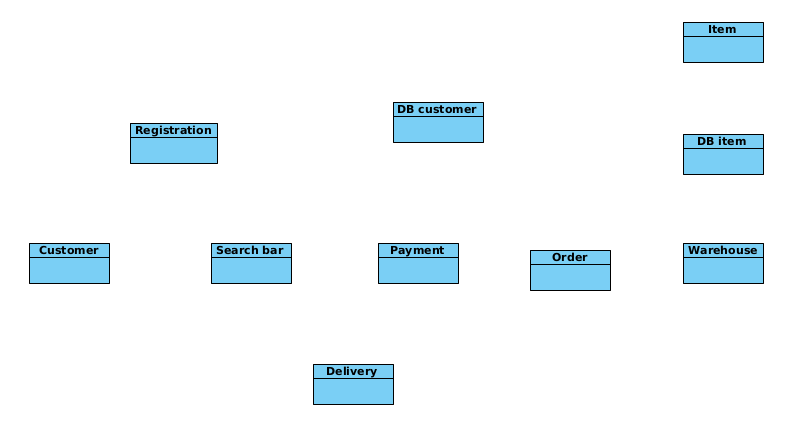
\includegraphics[width=0.8\textwidth]{Screenshot from 2023-04-03 13-30-37}
	\caption{Имена классов}
	\label{fig:classes}
\end{figure}

\section{Определение атрибутов классов}
Определим атрибуты для классов (рис.~\ref{fig:classes:atr}).

\begin{figure}[h!tp]
	\centering
	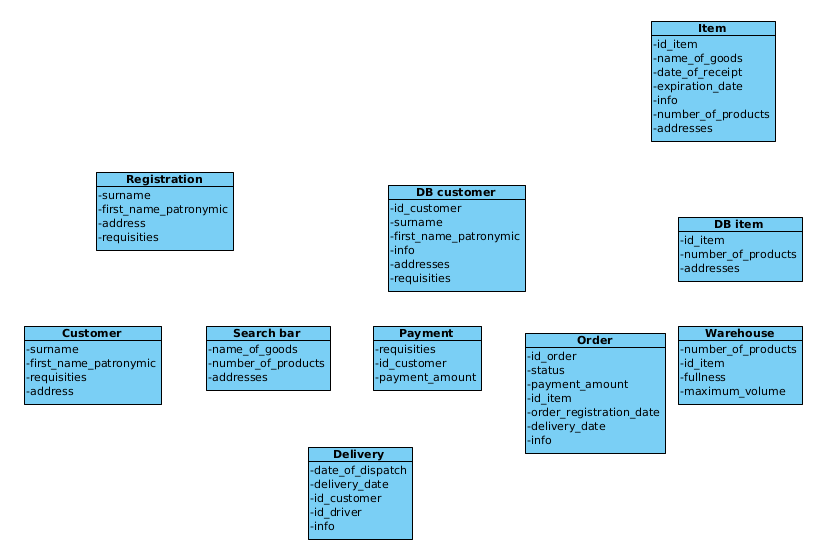
\includegraphics[width=0.8\textwidth]{Screenshot from 2023-04-03 13-38-40}
	\caption{Классы с атрибутами}
	\label{fig:classes:atr}
\end{figure}

\section{Добавление операций/методов классов}
Добавим операции/методы классов (рис.~\ref{fig:classes:methods}).

\begin{figure}[h!tp]
	\centering
	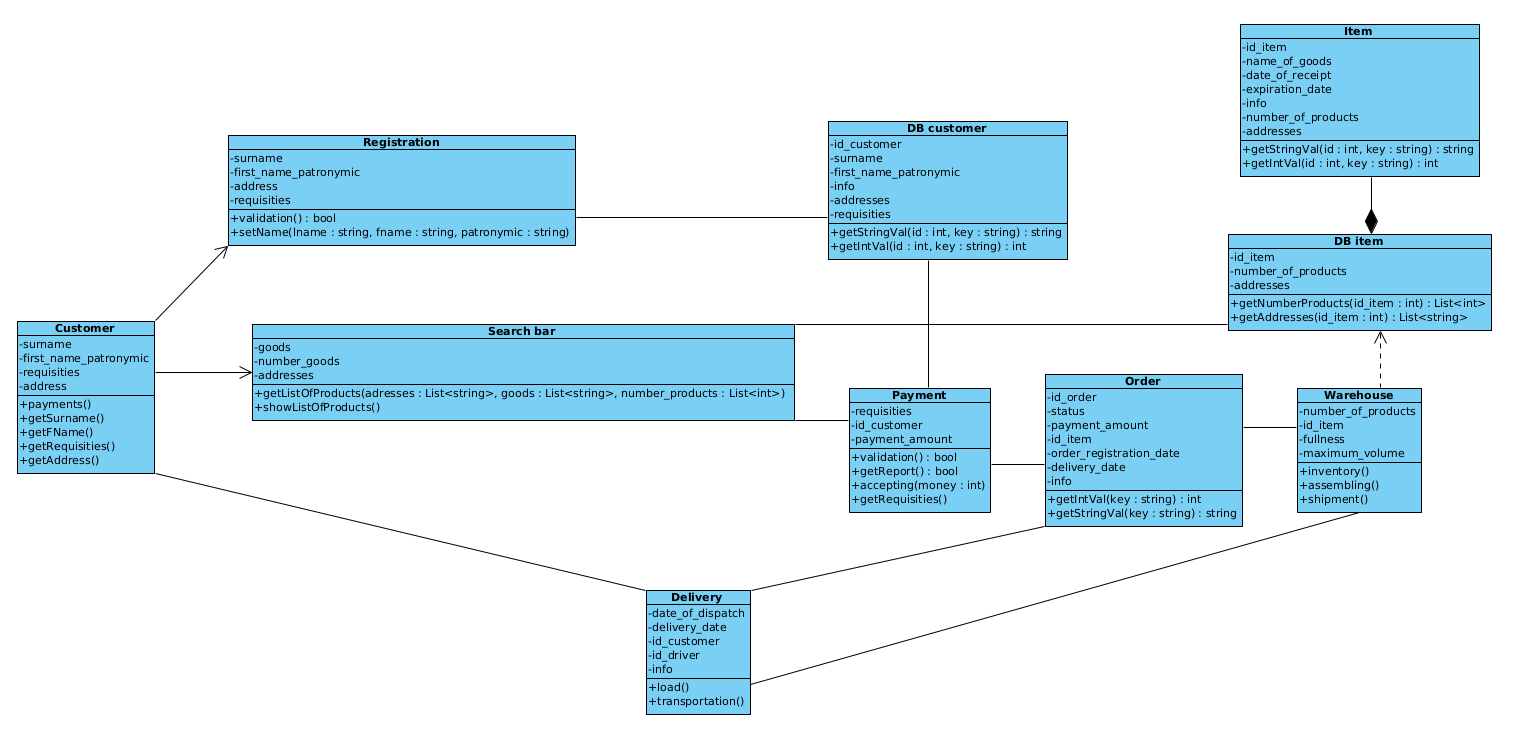
\includegraphics[width=0.8\textwidth]{Screenshot from 2023-04-03 14-38-21}
	\caption{Классы с атрибутами}
	\label{fig:classes:methods}
\end{figure}

\section{Отображение связей}
Отобразим связи между классами (рис.~\ref{fig:classes:link}).
Для этого рассмотрим различные отношения между классами на диаграмме.
В первую очередь добавим отношения ассоциации, затем остальные.

\begin{figure}[h!tp]
	\centering
	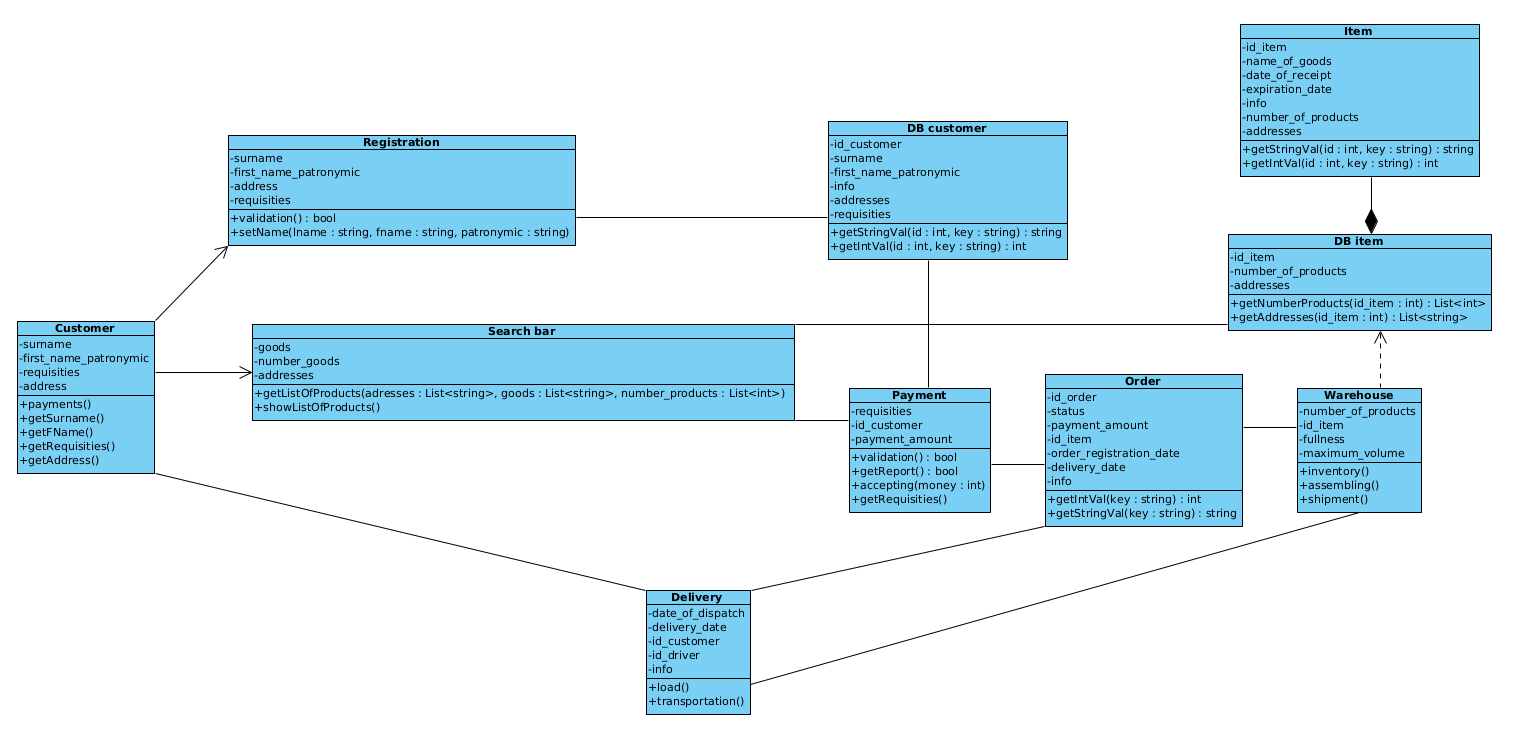
\includegraphics[width=0.8\textwidth]{Screenshot from 2023-04-03 14-38-21}
	\caption{Диаграмма классов с указанием связей}
	\label{fig:classes:link}
\end{figure}

Основные виды связей здесь определяются как ассоциативные. Только
\textit{Склад} зависит от \textit{Базы Данных товара}.
А класс \textit{Товар} является композицией класса
\textit{База Данных товаров}.

\section{Итоговая диаграмма}
Создадим итоговую диаграмму с указанием кратностей
(рис.~\ref{fig:classes:link}).

\begin{figure}[h!tp]
	\centering
	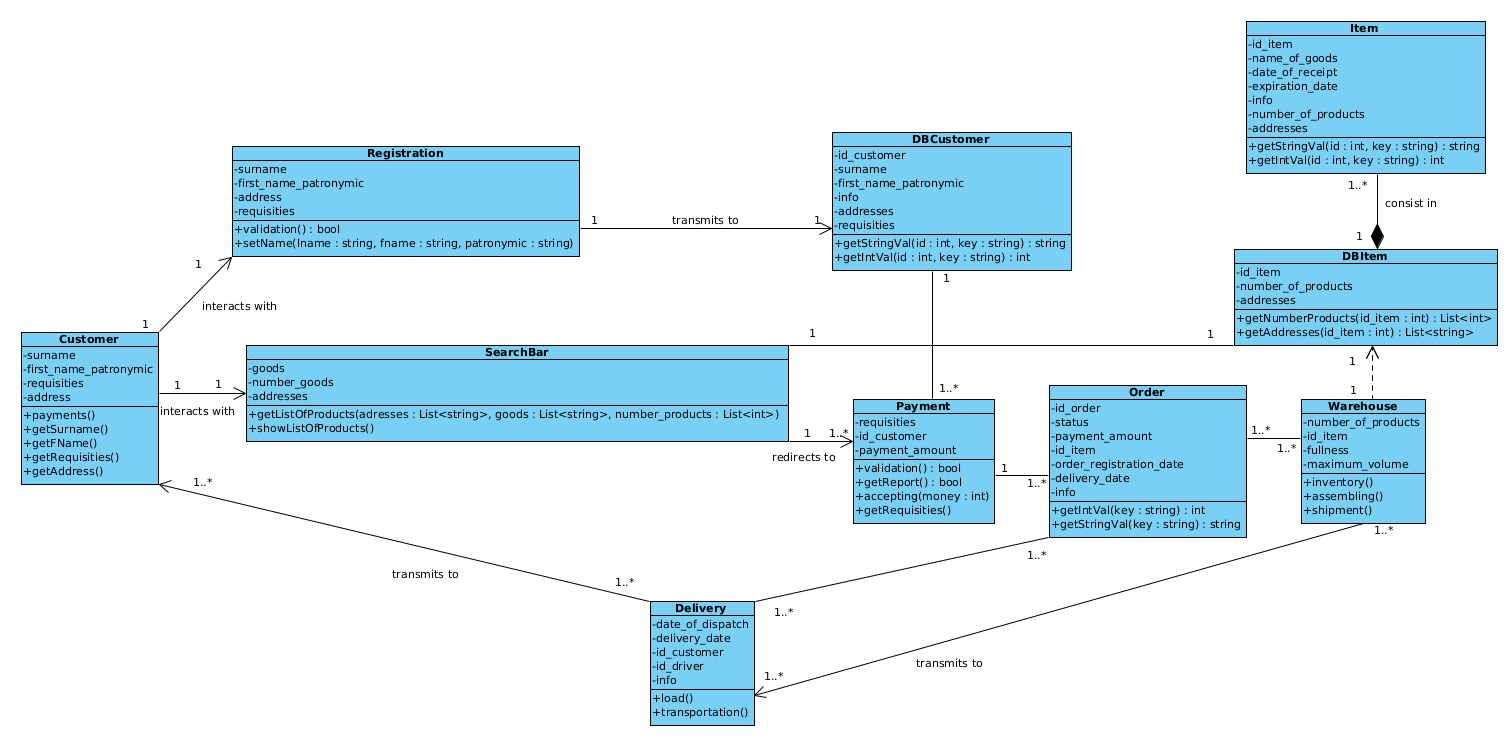
\includegraphics[width=1\textwidth]{Screenshot from 2023-04-04 17-59-45}
	\caption{Диаграмма классов с указанием связей}
	\label{fig:classes:link}
\end{figure}


\clearpage

\section*{Ответы на вопросы}
\addcontentsline{toc}{section}{Ответы на вопросы}

\begin{description}
	\item [Чем отличается класс уровня проектирования от класса
		уровня реализации?]
		На \textit{уровне проектирования} класс отражает основные проектные
		решения касательно распределения информации и планируемой
		функциональности, объединяя в себе сведения о состоянии и операциях.
		На \textit{уровне реализации} класс дорабатывается до такого вида,
		в каком он максимально удобен для воплощения в выбранной среде
		разработки,
		при этом не воспрещается опустить в нём те общие свойства,
		которые не применяются на выбранном языке программирования.
	\item [Опишите характеристики секции имени класса.]
		Верхняя часть диаграммы, в которой написано имя класса
		называется секцией имени. Секция имени имеет следующие
		характеристики:

		\begin{itemize}
			\item в качестве имени класса выбирается существительное в
				единственном числе;
			\item если имя класса состоит из нескольких слов, то оно
				записывается в верблюжьем стиле (от англ. "CamelCase");
			\item имя класса выравнивается по центру и пишется полужирным
				шрифтом;
			\item имя класса начинается с заглавной буквы;
			\item если класс абстрактный — то его имя пишется полужирным
				курсивом.
		\end{itemize}
	\item [Что собой представляет атрибут класса?]
		\textit{Атрибут} --- это свойство класса, которое может принимать
		множество значений. Множество допустимых значений атрибута образует
		домен. Атрибут имеет имя и отражает некоторое свойство моделируемой
		сущности, общее для всех объектов данного класса. Класс может иметь
		произвольное количество атрибутов.
	\item [Опишите характеристики секции атрибута класса.]
		Секция атрибутов имеет следующие характеристики:
		\begin{itemize}
			\item атрибуты выровнены по левому краю;
			\item атрибуты начинаются с маленькой буквы.
		\end{itemize}
	\item [Чем отличается абстрактный класс от статического класса?]
		\textit{Абстрактный класс} --- это класс, на основе которого нельзя
		создать объекты. Такие классы используются в качестве шаблона для
		дочерних классов при наследовании.
		\textit{Статический класс} --- это класс, в котором есть только
		статические поля и методы и на основе которого не создаются объекты.
	\item [Что собой представляет видимость атрибута?]
		\textbf{Видимость} указывает на то, что атрибут может быть прочитан
		или изменен с помощью объектов других классов. Причем, изменить
		можно только в том случае, если атрибут константой не является.
	\item [Что собой представляет тип атрибута?]
		\textbf{Тип} атрибута выбирается исходя из семантики значений,
		которые должны храниться в атрибуте, и, как правило, возможностей
		целевого языка программирования по представлению этих значений.
	\item [Что собой представляет кратность (множественность)?]
		\textbf{Кратность} атрибута характеризует количество значений,
		которые можно хранить в атрибуте.
	\item [Перечислите варианты указания кратности.]
		Варианты указания кратности:
		\begin{itemize}
			\item один к одному;
			\item один к многим;
			\item многие к одному;
			\item многие к многим.
		\end{itemize}
	\item [Что собой представляет модификатор?]
		\textbf{Модификатор} описывает особенности реализации атрибута.
	\item [Что собой представляет операция/методы класса?]
		\textit{Операция/методы} --- реализация функции, которую можно
		запросить у любого объекта класса. Операция показывает,
		что можно сделать с объектом.
	\item [Опишите характеристики секции методов класса.]
		Секция операций/методов имеет следующие характеристики:
		\begin{itemize}
			\item операции/методы выровнены по левому краю;
			\item операции/методы пишутся с маленькой буквы.
		\end{itemize}
	\item [Опишите набор спецификаций методов.]
		\begin{itemize}
			\item "+"/Public – указывает на общедоступность атрибута
				как для чтения, так и и модификации атрибутами других классов;
			\item "\#"/Protected – указывает на защищенность атрибута,
				когда он доступен только объектам текущего класса,
				а также его потомкам;
			\item "–"/Private – указывает на закрытость атрибута,
				когда доступность атрибута обеспечивается объектам текущего
				класса;
			\item "~"/ Package – указывает на доступность атрибут только
				объектам классов текущего пакета.
		\end{itemize}
	\item [Что собой представляет тип параметра?]
		Тип выбирается исходя из семантики значений, которые должны
		храниться, и, как правило, возможностей
		целевого языка программирования по представлению этих значений.
	\item [Что собой представляет тип метода?]
		Тип выбирается исходя из семантики значений, которые должны
		возвращаться из метода, и, как правило, возможностей
		целевого языка программирования по представлению этих значений.
	\item [Чем отличается тип параметра от типа метода?]
		Тип параметра задает как он будет храниться, а метода, что будет
		возвращать.
	\item [О чем могут сказать свойства метода?]
		Какие аргументы он принемает и какого типа значение возвращает.
	\item [Перечислите основные виды операций.]
		Существуют следующие виды операций (методов):
		\begin{itemize}
			\item конструктор;
			\item деструктор;
			\item модификатор;
			\item селектор;
			\item итератор;
			\item событие.
		\end{itemize}
	\item [Опишите алгоритм создания диаграмм классов
		проектирования.]
		Алгоритм:
		\begin{enumerate}
			\item Наметить основные классы.
			\item Изобразить классы на диаграмме.
			\item Определить виды классов.
			\item Определить атрибуты для классов.
			\item Добавить операции/методы классов.
			\item Отобразить связи между классами.
			\item Создать итоговую диаграмму с указанием кратностей.
		\end{enumerate}

\end{description}

\clearpage

\section*{\LARGE Вывод}
\addcontentsline{toc}{section}{Вывод}
Мы создали диаграмму классов детального уровня.
Для этого определили сем классов для построения диаграммы: Customer,
Registration, SearchBar, DBCustomer, Item, DBItem, Payment, Order, Warehouse,
Delivery. Добавили атрибуты и описали методы, установили отношения между
классами, указали кратности.
Основные отношения между классами --- ассоциация. Класс Warehouse и
DBItem связаны между собой отношением зависимости.
А класс DBItem связан с Item связью --- композиция. Создадим таблицы
(табл.~\ref{tabular:descriptions}\,-\,\ref{tabular:interactions})
для наглядного анализа диаграммы.

\begin{table}[h!tp]
	\centering
	\caption{\leftline{Описание классов диаграммы}}
	\label{tabular:descriptions}
	\begin{tabular}{|p{0.35\textwidth}|p{0.65\textwidth}|}
		\hline \textbf{Название класса} & \textbf{Описание} \\ \hline
		Customer & Класс для представления интерфейса пользователя \\ \hline
		Registration & Класс для регистрации пользователя в системе \\ \hline
		SearchBar & Класс для представляющий интерфейс сайта
			для пользователя \\ \hline
		DBCustomer & Класс для работы c базой данных клиентов \\ \hline
		Item & Класс для представления товара в базе данных \\ \hline
		DBItem & Класс для работы c базой данных товара \\ \hline
		Payment & Класс для оплаты \\ \hline
		Order & Класс для представления заказа \\ \hline
		Warehouse & Класс для представления склада \\ \hline
		Delivery & Класс для представления интерфейс доставки\\ \hline
	\end{tabular}
\end{table}

\begin{longtable}{|p{0.2\textwidth}
	|p{0.25\textwidth}
	|p{0.25\textwidth}
	|p{0.2\textwidth}
	|}
	\caption{\leftline{Взаимодействие между классами}}
	\label{tabular:interactions}\\

	\hline \textbf{Класс} & \textbf{Кратность}
		& \textbf{Тип отношений} & \textbf{Класс} \\ \hline
	\endhead

	Customer & Один к одному & ассоциация & Registration \\ \hline
	Customer & Один к одному & ассоциация & SearchBar \\ \hline
	Registration & Один к одному & ассоциация & DBCustomer \\ \hline
	SearchBar & Один к одному & ассоциация & DBItem \\ \hline
	SearchBar & Один к многим & ассоциация & Payment \\ \hline
	DBCustomer & Один к многим & ассоциация & Payment \\ \hline
	DBItem & Один к многим & композиция & Item \\ \hline
	Payment & Один к многим & ассоциация & Order \\ \hline
	Order & Многие к многим & ассоциация & Warehouse \\ \hline
	Order & Многие к многим & ассоциация & Delivery \\ \hline
	Warehouse & Один к одному & зависимость & DBItem \\ \hline
	Warehouse & Многие к многим & ассоциация & Delivery \\ \hline
	Delivery & Один к многим & ассоциация & Customer \\ \hline
\end{longtable}

